% Options for packages loaded elsewhere
\PassOptionsToPackage{unicode}{hyperref}
\PassOptionsToPackage{hyphens}{url}
\PassOptionsToPackage{dvipsnames,svgnames,x11names}{xcolor}
%
\documentclass[
  ignorenonframetext,
]{beamer}
\usepackage{pgfpages}
\setbeamertemplate{caption}[numbered]
\setbeamertemplate{caption label separator}{: }
\setbeamercolor{caption name}{fg=normal text.fg}
\beamertemplatenavigationsymbolsempty
% Prevent slide breaks in the middle of a paragraph
\widowpenalties 1 10000
\raggedbottom
\setbeamertemplate{part page}{
  \centering
  \begin{beamercolorbox}[sep=16pt,center]{part title}
    \usebeamerfont{part title}\insertpart\par
  \end{beamercolorbox}
}
\setbeamertemplate{section page}{
  \centering
  \begin{beamercolorbox}[sep=12pt,center]{part title}
    \usebeamerfont{section title}\insertsection\par
  \end{beamercolorbox}
}
\setbeamertemplate{subsection page}{
  \centering
  \begin{beamercolorbox}[sep=8pt,center]{part title}
    \usebeamerfont{subsection title}\insertsubsection\par
  \end{beamercolorbox}
}
\AtBeginPart{
  \frame{\partpage}
}
\AtBeginSection{
  \ifbibliography
  \else
    \frame{\sectionpage}
  \fi
}
\AtBeginSubsection{
  \frame{\subsectionpage}
}
\usepackage{amsmath,amssymb}
\usepackage{lmodern}
\usepackage{iftex}
\ifPDFTeX
  \usepackage[T1]{fontenc}
  \usepackage[utf8]{inputenc}
  \usepackage{textcomp} % provide euro and other symbols
\else % if luatex or xetex
  \usepackage{unicode-math}
  \defaultfontfeatures{Scale=MatchLowercase}
  \defaultfontfeatures[\rmfamily]{Ligatures=TeX,Scale=1}
\fi
% Use upquote if available, for straight quotes in verbatim environments
\IfFileExists{upquote.sty}{\usepackage{upquote}}{}
\IfFileExists{microtype.sty}{% use microtype if available
  \usepackage[]{microtype}
  \UseMicrotypeSet[protrusion]{basicmath} % disable protrusion for tt fonts
}{}
\makeatletter
\@ifundefined{KOMAClassName}{% if non-KOMA class
  \IfFileExists{parskip.sty}{%
    \usepackage{parskip}
  }{% else
    \setlength{\parindent}{0pt}
    \setlength{\parskip}{6pt plus 2pt minus 1pt}}
}{% if KOMA class
  \KOMAoptions{parskip=half}}
\makeatother
\usepackage{xcolor}
\newif\ifbibliography
\setlength{\emergencystretch}{3em} % prevent overfull lines
\providecommand{\tightlist}{%
  \setlength{\itemsep}{0pt}\setlength{\parskip}{0pt}}
\setcounter{secnumdepth}{-\maxdimen} % remove section numbering

\usepackage{textpos}
\setbeamertemplate{headline}{
  \begin{textblock*}{5cm}(10.2cm,0.2cm)
  
\includegraphics[width=2.2cm]{UniUrb-logo.png}
  \end{textblock*}}
  
  \definecolor{myblue}{HTML}{005997}
  \setbeamercolor{frametitle}{fg=myblue}
    \setbeamercolor{framesubtitle}{fg=myblue}
    \setbeamercolor{frametitle right}{fg=myblue}
  \setbeamercolor{titlelike}{fg=myblue}
    \setbeamercolor{title}{fg=myblue}
      \setbeamercolor{subtitle}{fg=myblue}
    \setbeamercolor{part title}{fg=myblue}
    \setbeamercolor{section title}{fg=myblue}
    \setbeamercolor{subsection title}{fg=myblue}
  \setbeamercolor{section name}{fg=myblue}
  \setbeamercolor{subsection name}{fg=myblue}
  \setbeamercolor{part name}{fg=myblue}
  \setbeamercolor{title in head/foot}{fg=myblue}
  \setbeamercolor{subtitle in head/foot}{fg=myblue}
  \setbeamercolor{block title}{fg=myblue}
  
  \setbeamercolor{bullet}{fg=myblue}
  \setbeamercolor{section in toc}{fg=myblue}
  \setbeamercolor{subsection in toc}{fg=myblue}
  \setbeamercolor{section in head/foot}{fg=myblue}
  \setbeamercolor{subsection in head/foot}{fg=myblue}
  
  
  \setbeamercolor{itemize item}{fg = myblue}
  \setbeamercolor{itemize subitem}{fg = myblue}
  \setbeamercolor{itemize subsubitem}{fg = myblue}
  \setbeamercolor{enumerate item}{fg = myblue}
  \setbeamercolor{enumerate subitem}{fg = myblue}
  \setbeamercolor{enumerate subsubitem}{fg = myblue}
  
 
  
\usepackage{etoolbox}
\AtBeginEnvironment{thebibliography}{\scriptsize}
\ifLuaTeX
  \usepackage{selnolig}  % disable illegal ligatures
\fi
\usepackage[round]{natbib}
\bibliographystyle{apalike}
\IfFileExists{bookmark.sty}{\usepackage{bookmark}}{\usepackage{hyperref}}
\IfFileExists{xurl.sty}{\usepackage{xurl}}{} % add URL line breaks if available
\urlstyle{same} % disable monospaced font for URLs
\hypersetup{
  pdftitle={Introductory Workshop to Bibliometrics},
  pdfauthor={Luis Carlos Castillo},
  colorlinks=true,
  linkcolor={myblue},
  filecolor={Maroon},
  citecolor={Blue},
  urlcolor={Blue},
  pdfcreator={LaTeX via pandoc}}

\title{Introductory Workshop to Bibliometrics}
\author{Luis Carlos Castillo}
\date{01 June 2023}
\institute{University of Urbino\\
Ph.D.~Program in Global Studies}

\begin{document}
\frame{\titlepage}

\begin{frame}{Introduction}
\protect\hypertarget{introduction}{}
\begin{itemize}
\item
  This section will provide an overview of bibliometrics and the
  importance of bibliometric analysis.
\item
  Search in the Web of Science and Scopus platforms.
\item
  Identify different tools but focusing on R programming language.
\end{itemize}
\end{frame}

\begin{frame}{What is Bibliometrics?}
\protect\hypertarget{what-is-bibliometrics}{}
Following \citet{donthu2021}, \citet{ellegaard2015}, \citet{Aria2017},
and \citet{bornmann2015} bibliometric analysis:

\begin{itemize}
\tightlist
\item
  Is a methodology that applies quantitative techniques to bibliographic
  data and plays a vital role in evaluating research output.
\item
  This technique allows researchers to uncover emerging trends
  identifying knowledge gaps in specific domains and analyze a
  significant quantity of documents .
\item
  It offers three types of analysis: performance analysis, science
  mapping, and network analysis.
\end{itemize}
\end{frame}

\begin{frame}{Types of Analysis I}
\protect\hypertarget{types-of-analysis-i}{}
\begin{block}{Performance Analysis}
\protect\hypertarget{performance-analysis}{}
\begin{center}
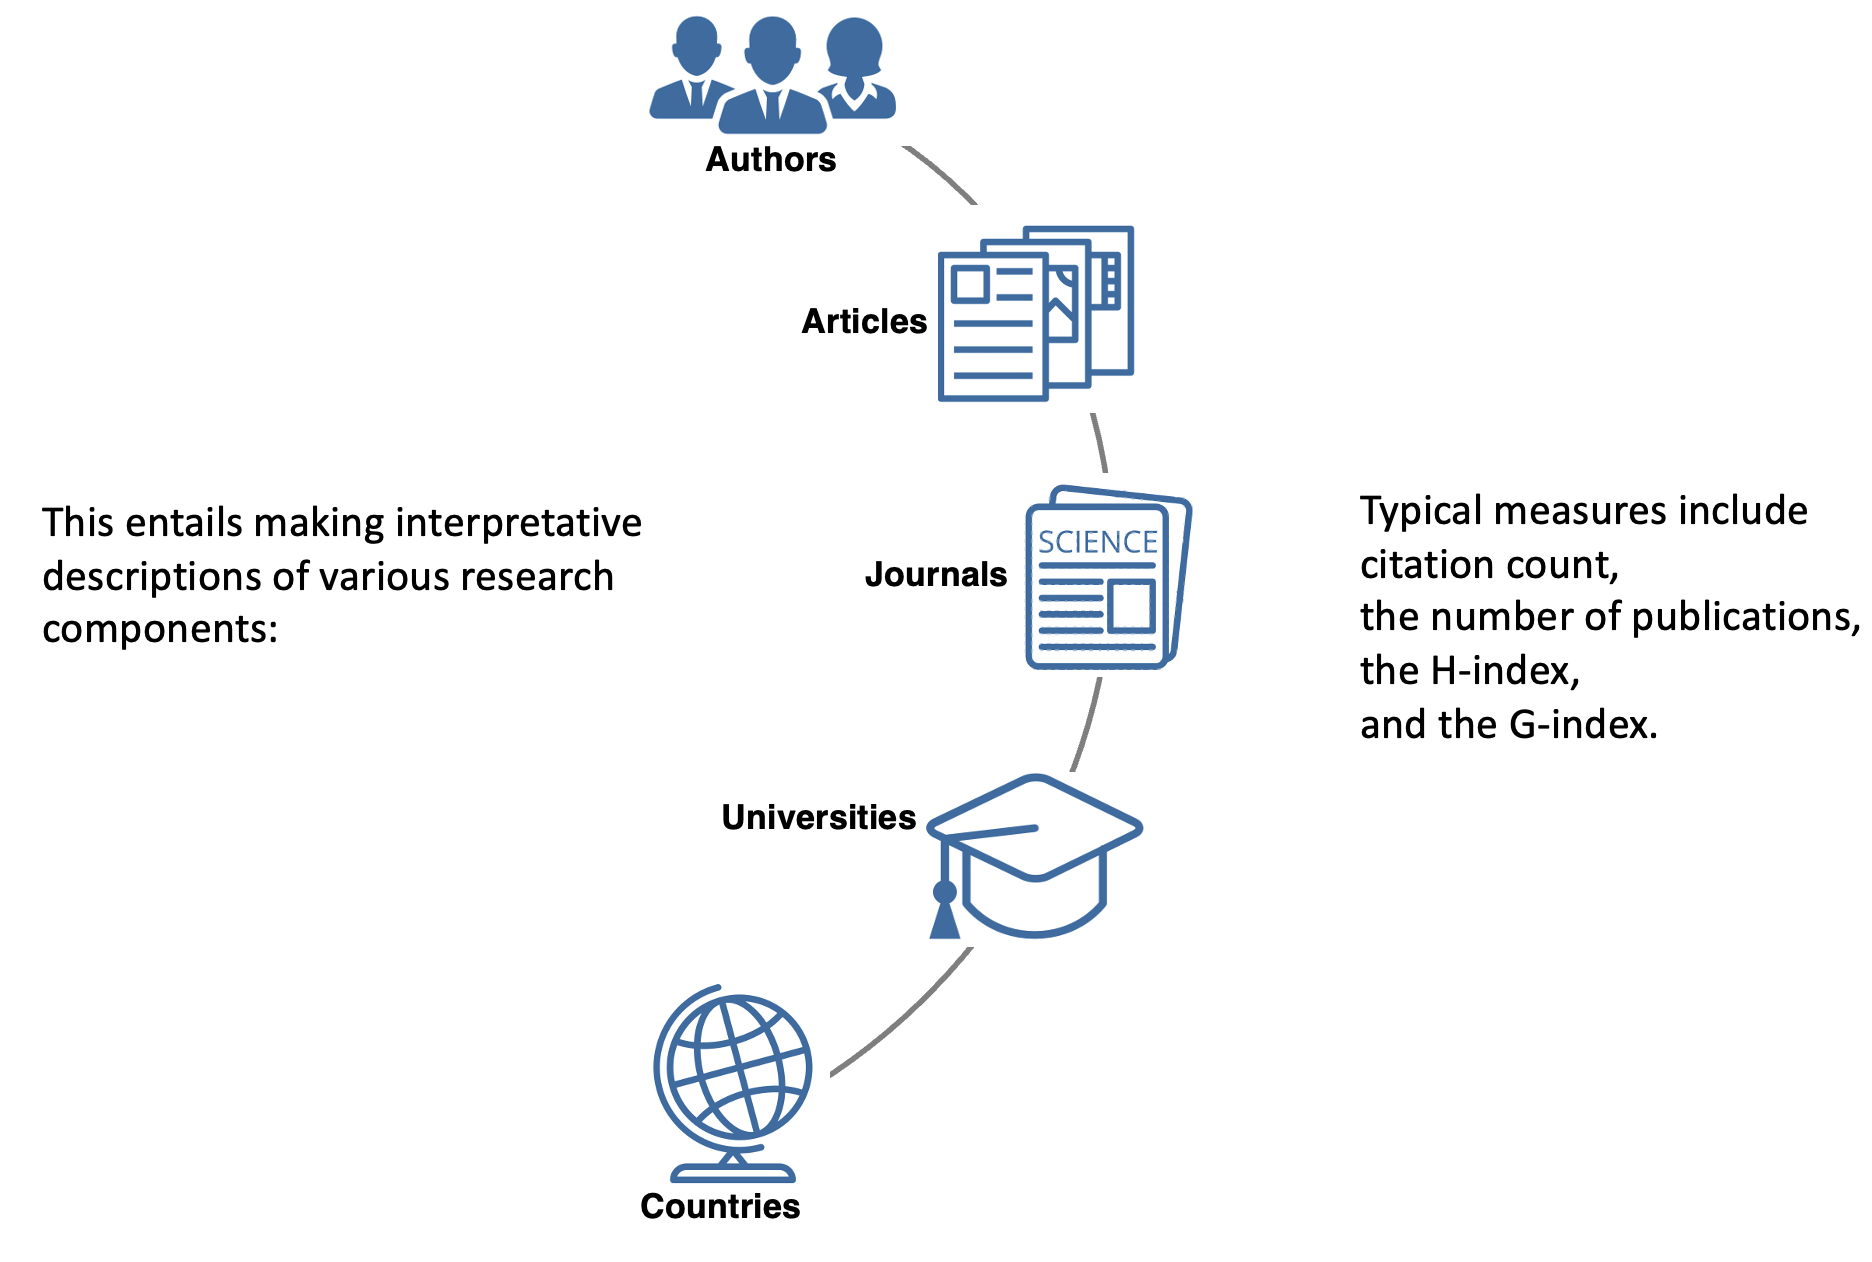
\includegraphics[width=1\textwidth]{pic_1.png}
\end{center}
\end{block}
\end{frame}

\begin{frame}{Types of Analysis II}
\protect\hypertarget{types-of-analysis-ii}{}
\begin{block}{Science Mapping}
\protect\hypertarget{science-mapping}{}
\begin{center}
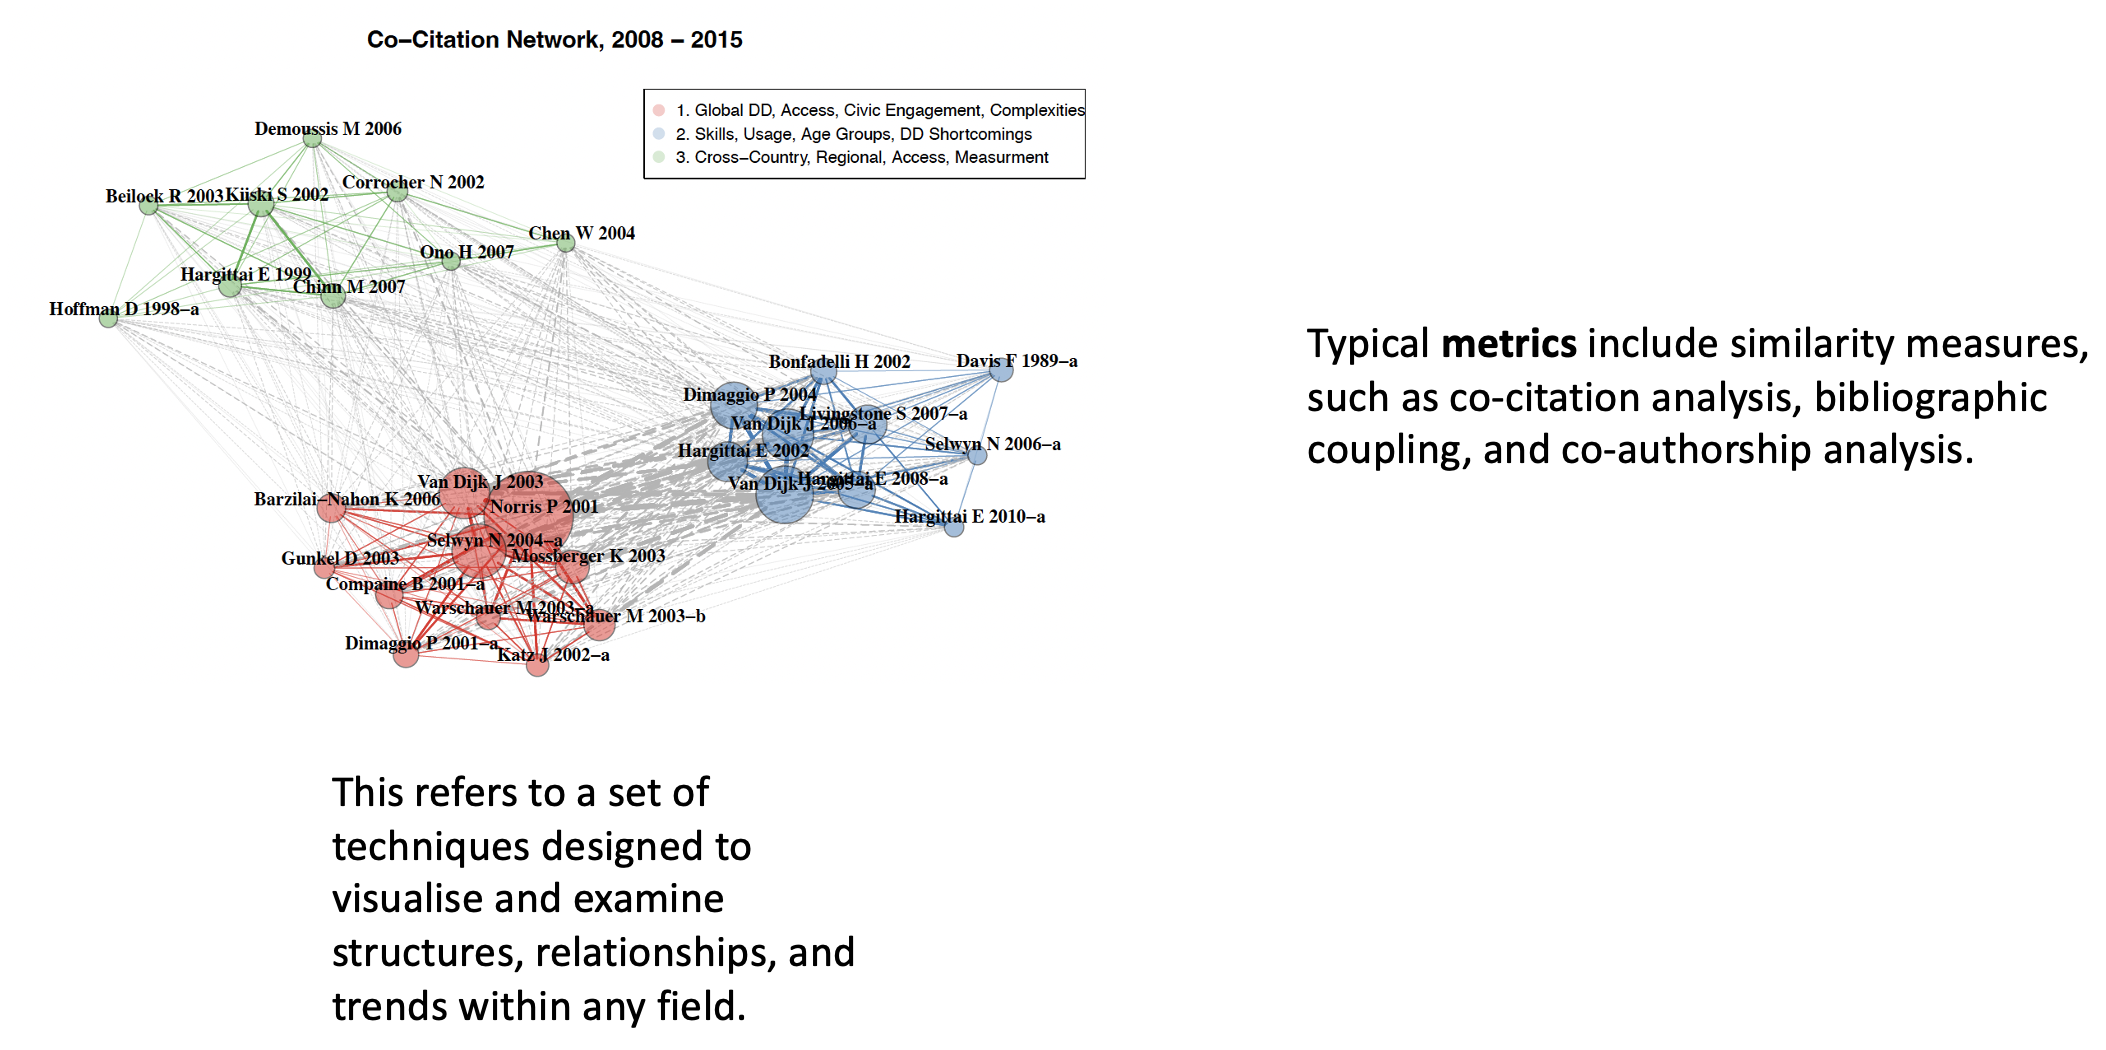
\includegraphics[width=1\textwidth]{pic_2.png}
\end{center}
\end{block}
\end{frame}

\begin{frame}{Types of Analysis III}
\protect\hypertarget{types-of-analysis-iii}{}
\begin{block}{Network Analysis}
\protect\hypertarget{network-analysis}{}
\begin{center}
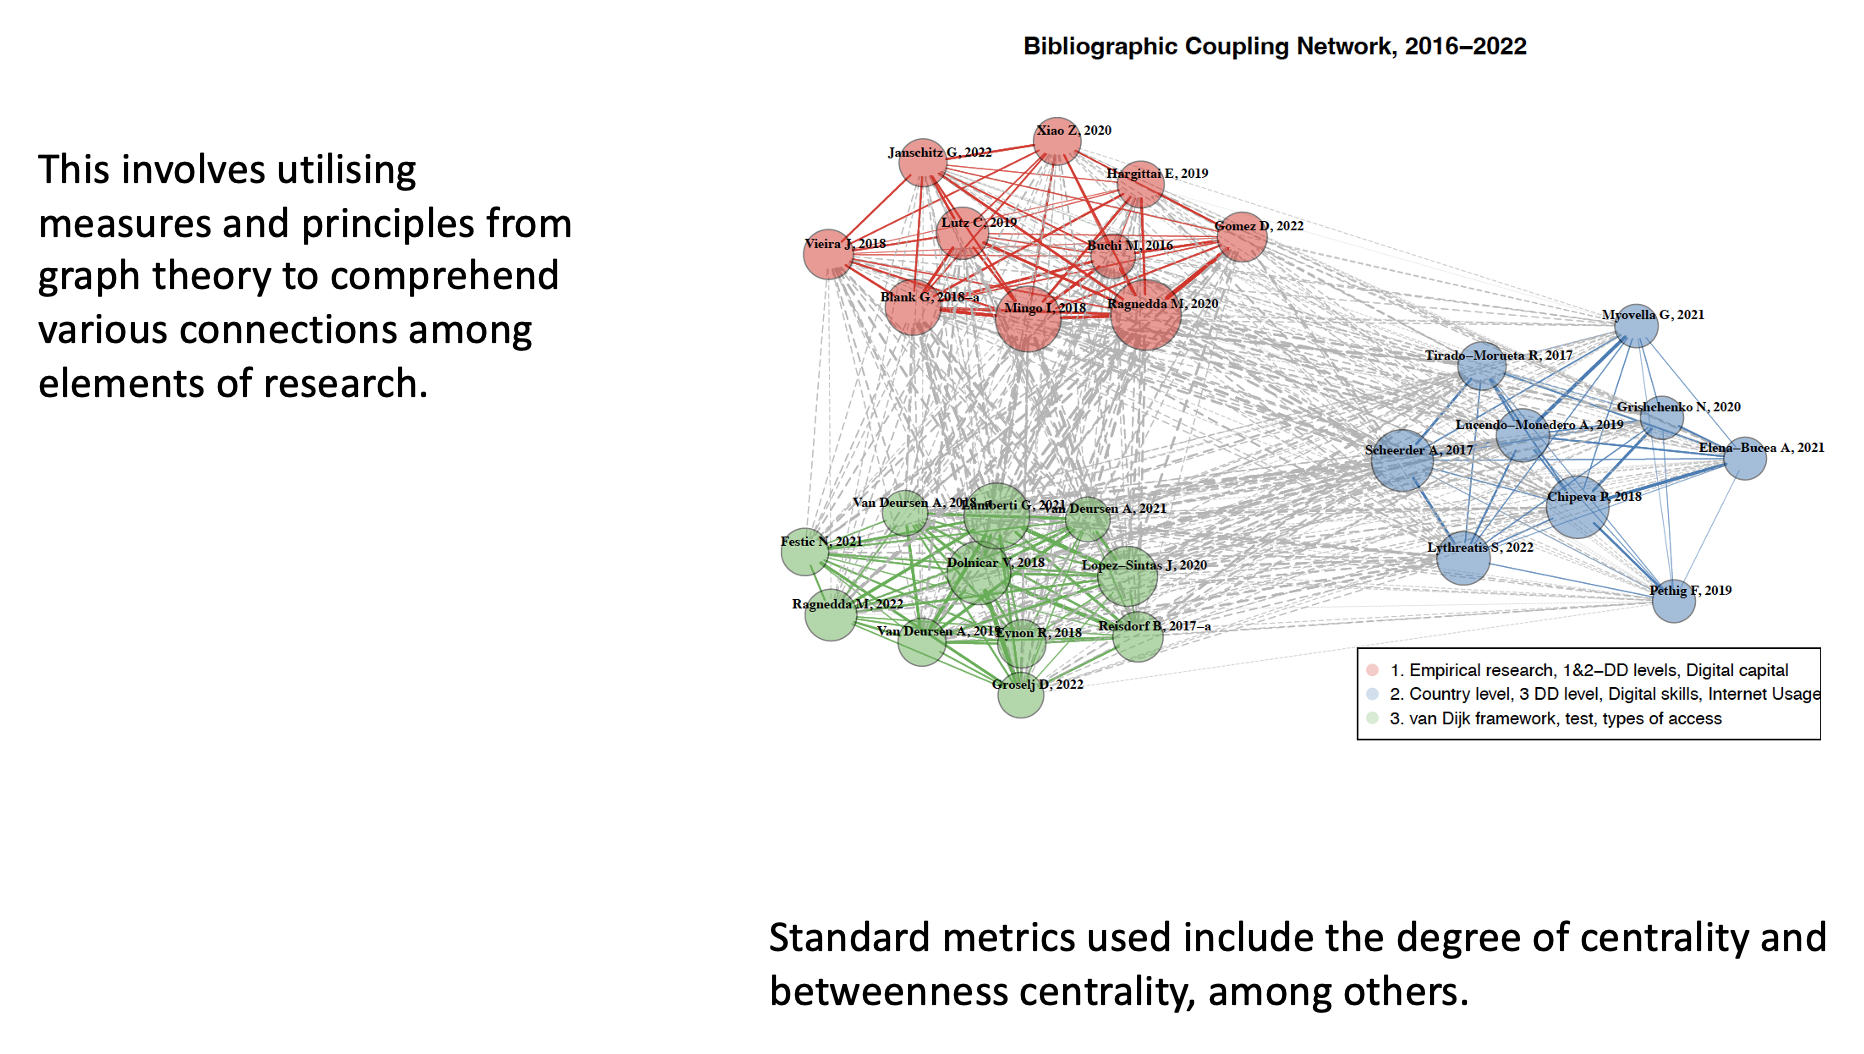
\includegraphics[width=1\textwidth]{pic_3.png}
\end{center}
\end{block}
\end{frame}

\begin{frame}{Why is it important?}
\protect\hypertarget{why-is-it-important}{}
\begin{itemize}
\tightlist
\item
  Identifying Relevant Literature
\item
  Assessing Research Impact
\item
  Understanding Research Trends and Relationships
\item
  Choosing Where to Publish
\item
  Choosing Where to Do Research
\end{itemize}
\end{frame}

\begin{frame}{Limitations}
\protect\hypertarget{limitations}{}
\begin{itemize}
\item
  Citations bias
\item
  Bibliometrics does not replace in-depth reading the literature
\item
  The Mathew effect
\end{itemize}
\end{frame}

\begin{frame}{The role of digital platforms I}
\protect\hypertarget{the-role-of-digital-platforms-i}{}
\begin{block}{Digital libraries}
\protect\hypertarget{digital-libraries}{}
\begin{center}
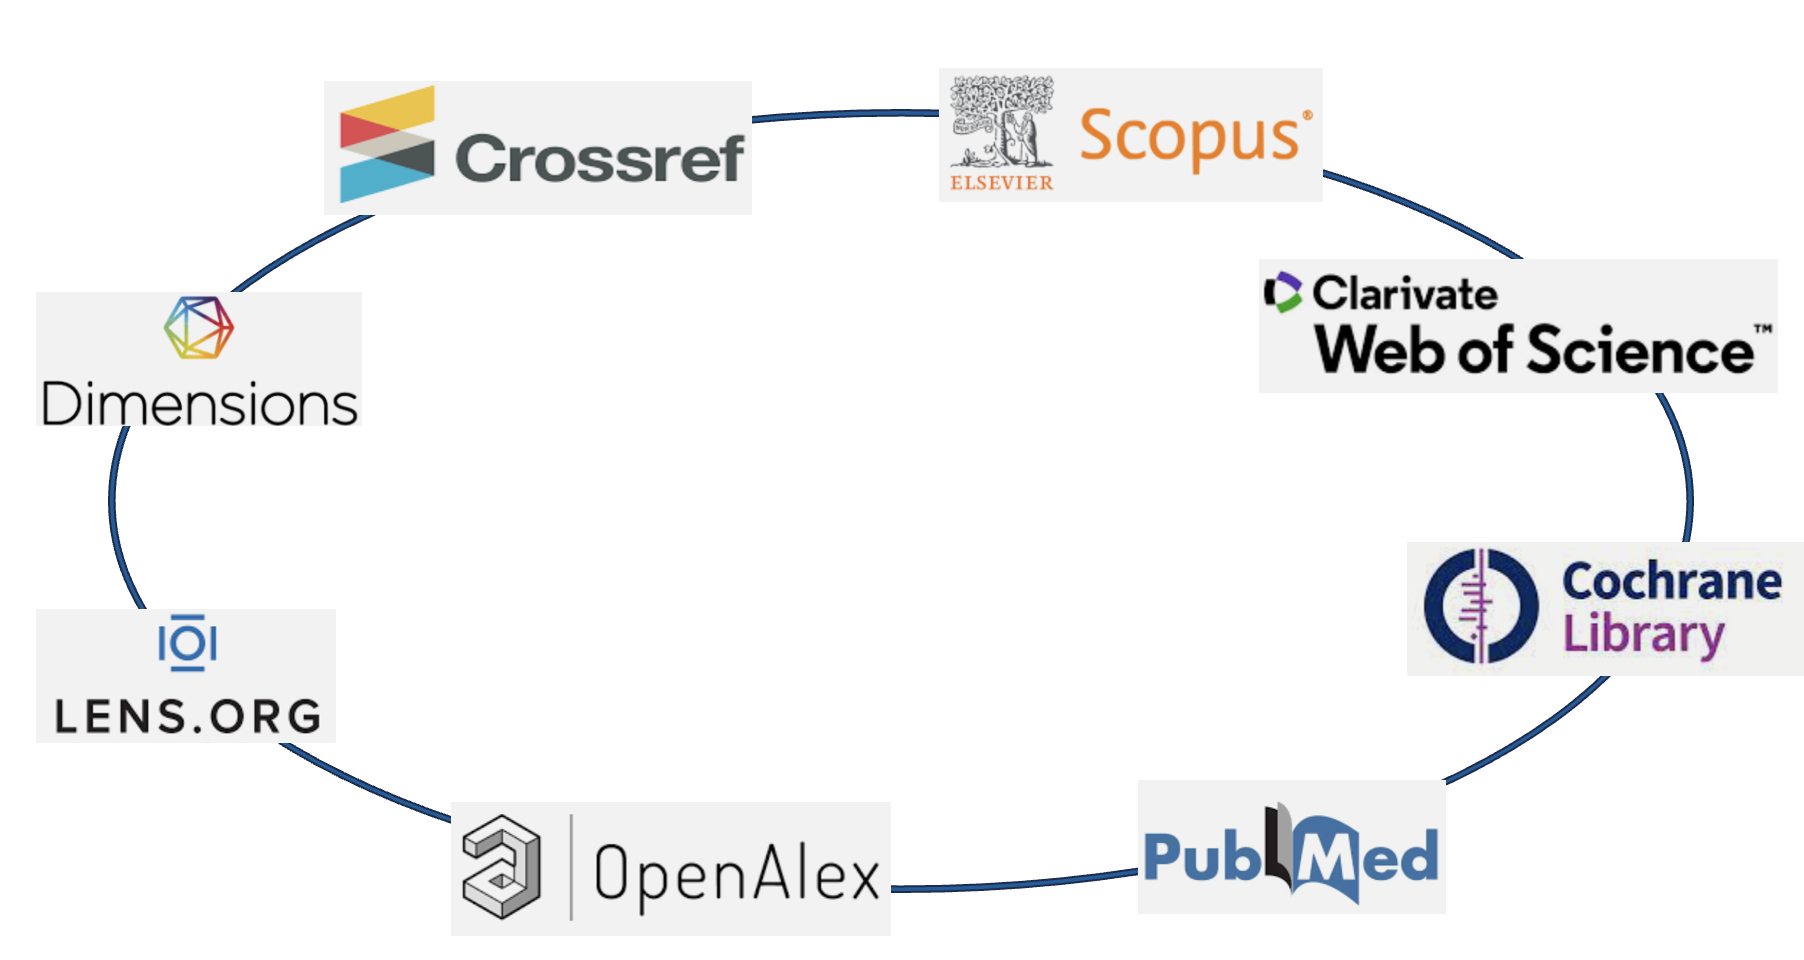
\includegraphics[width=1\textwidth]{pic_4.png}
\end{center}
\end{block}
\end{frame}

\begin{frame}{The Web of Science and Scopus}
\protect\hypertarget{the-web-of-science-and-scopus}{}
\begin{itemize}
\item
  Integrating Web of Science and Scopus databases is complex and
  requires a structured workflow, as pointed out by
  \citet{echchakoui2020} and \citet{caputo2022}.
\item
  Merging these databases can help mitigate resource bias in research.
  However, other biases such as retrieval bias and medium bias may
  persist.
\end{itemize}
\end{frame}

\begin{frame}{Hands-On The Data}
\protect\hypertarget{hands-on-the-data}{}
Please open the \href{https://www.uniurb.it/}{University of Urbino
Website} and enter with your credentials to the Web of Science and
Scopus platforms.

Google Drive Repository
\href{https://drive.google.com/drive/folders/1Mw6cWYZZxRlZTQAUYZofifyY_xkmcVeK}{\emph{Introductory
Workshop to Bibliometrics}}\emph{.}
\end{frame}

\renewcommand\refname{References}
\begin{frame}[allowframebreaks]{References}
  \bibliographytrue
  \bibliography{references.bib}
\end{frame}

\end{document}
